\subsection*{Supplementary Results}

\begin{figure}[htbp]
    \centering
    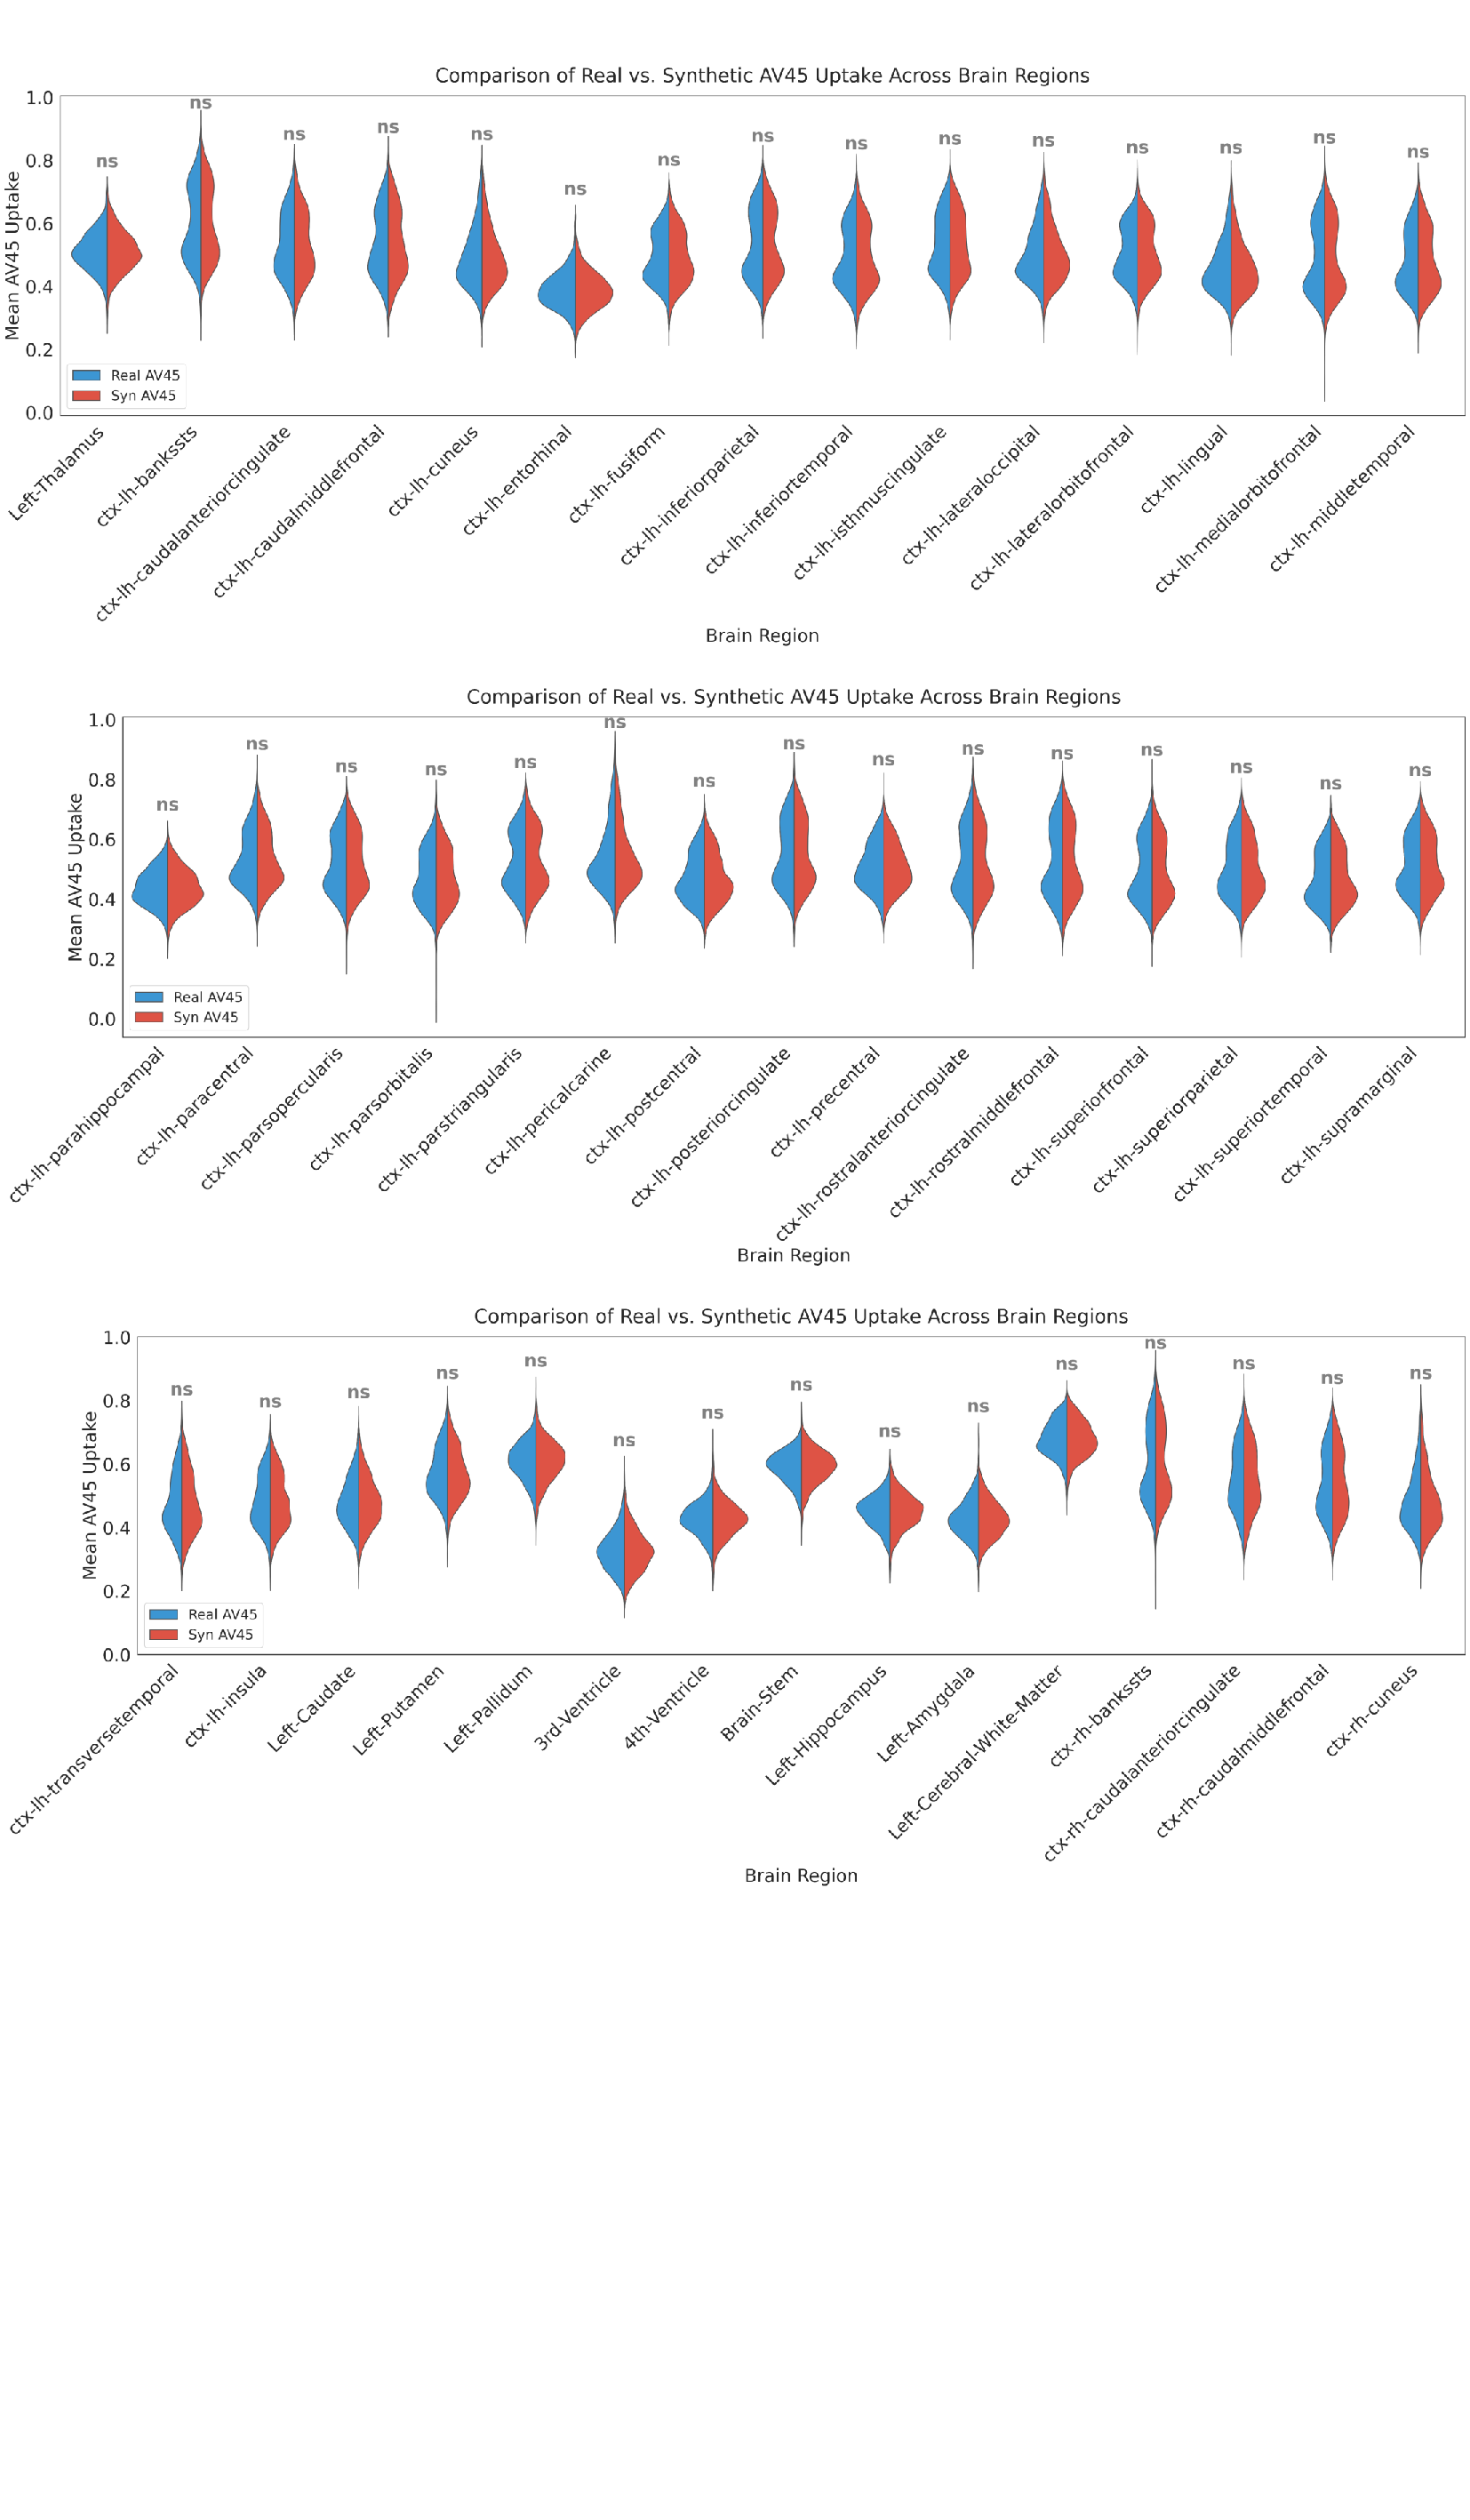
\includegraphics[width=\textwidth]{supplementary_figure_1}
    \caption{\textbf{Comparison of real and synthetic AV45 uptake across the remaining brain regions (Part 1 of 2).}}
    \label{fig:supp_av45_1}
\end{figure}

\begin{figure}[htbp]
    \centering
    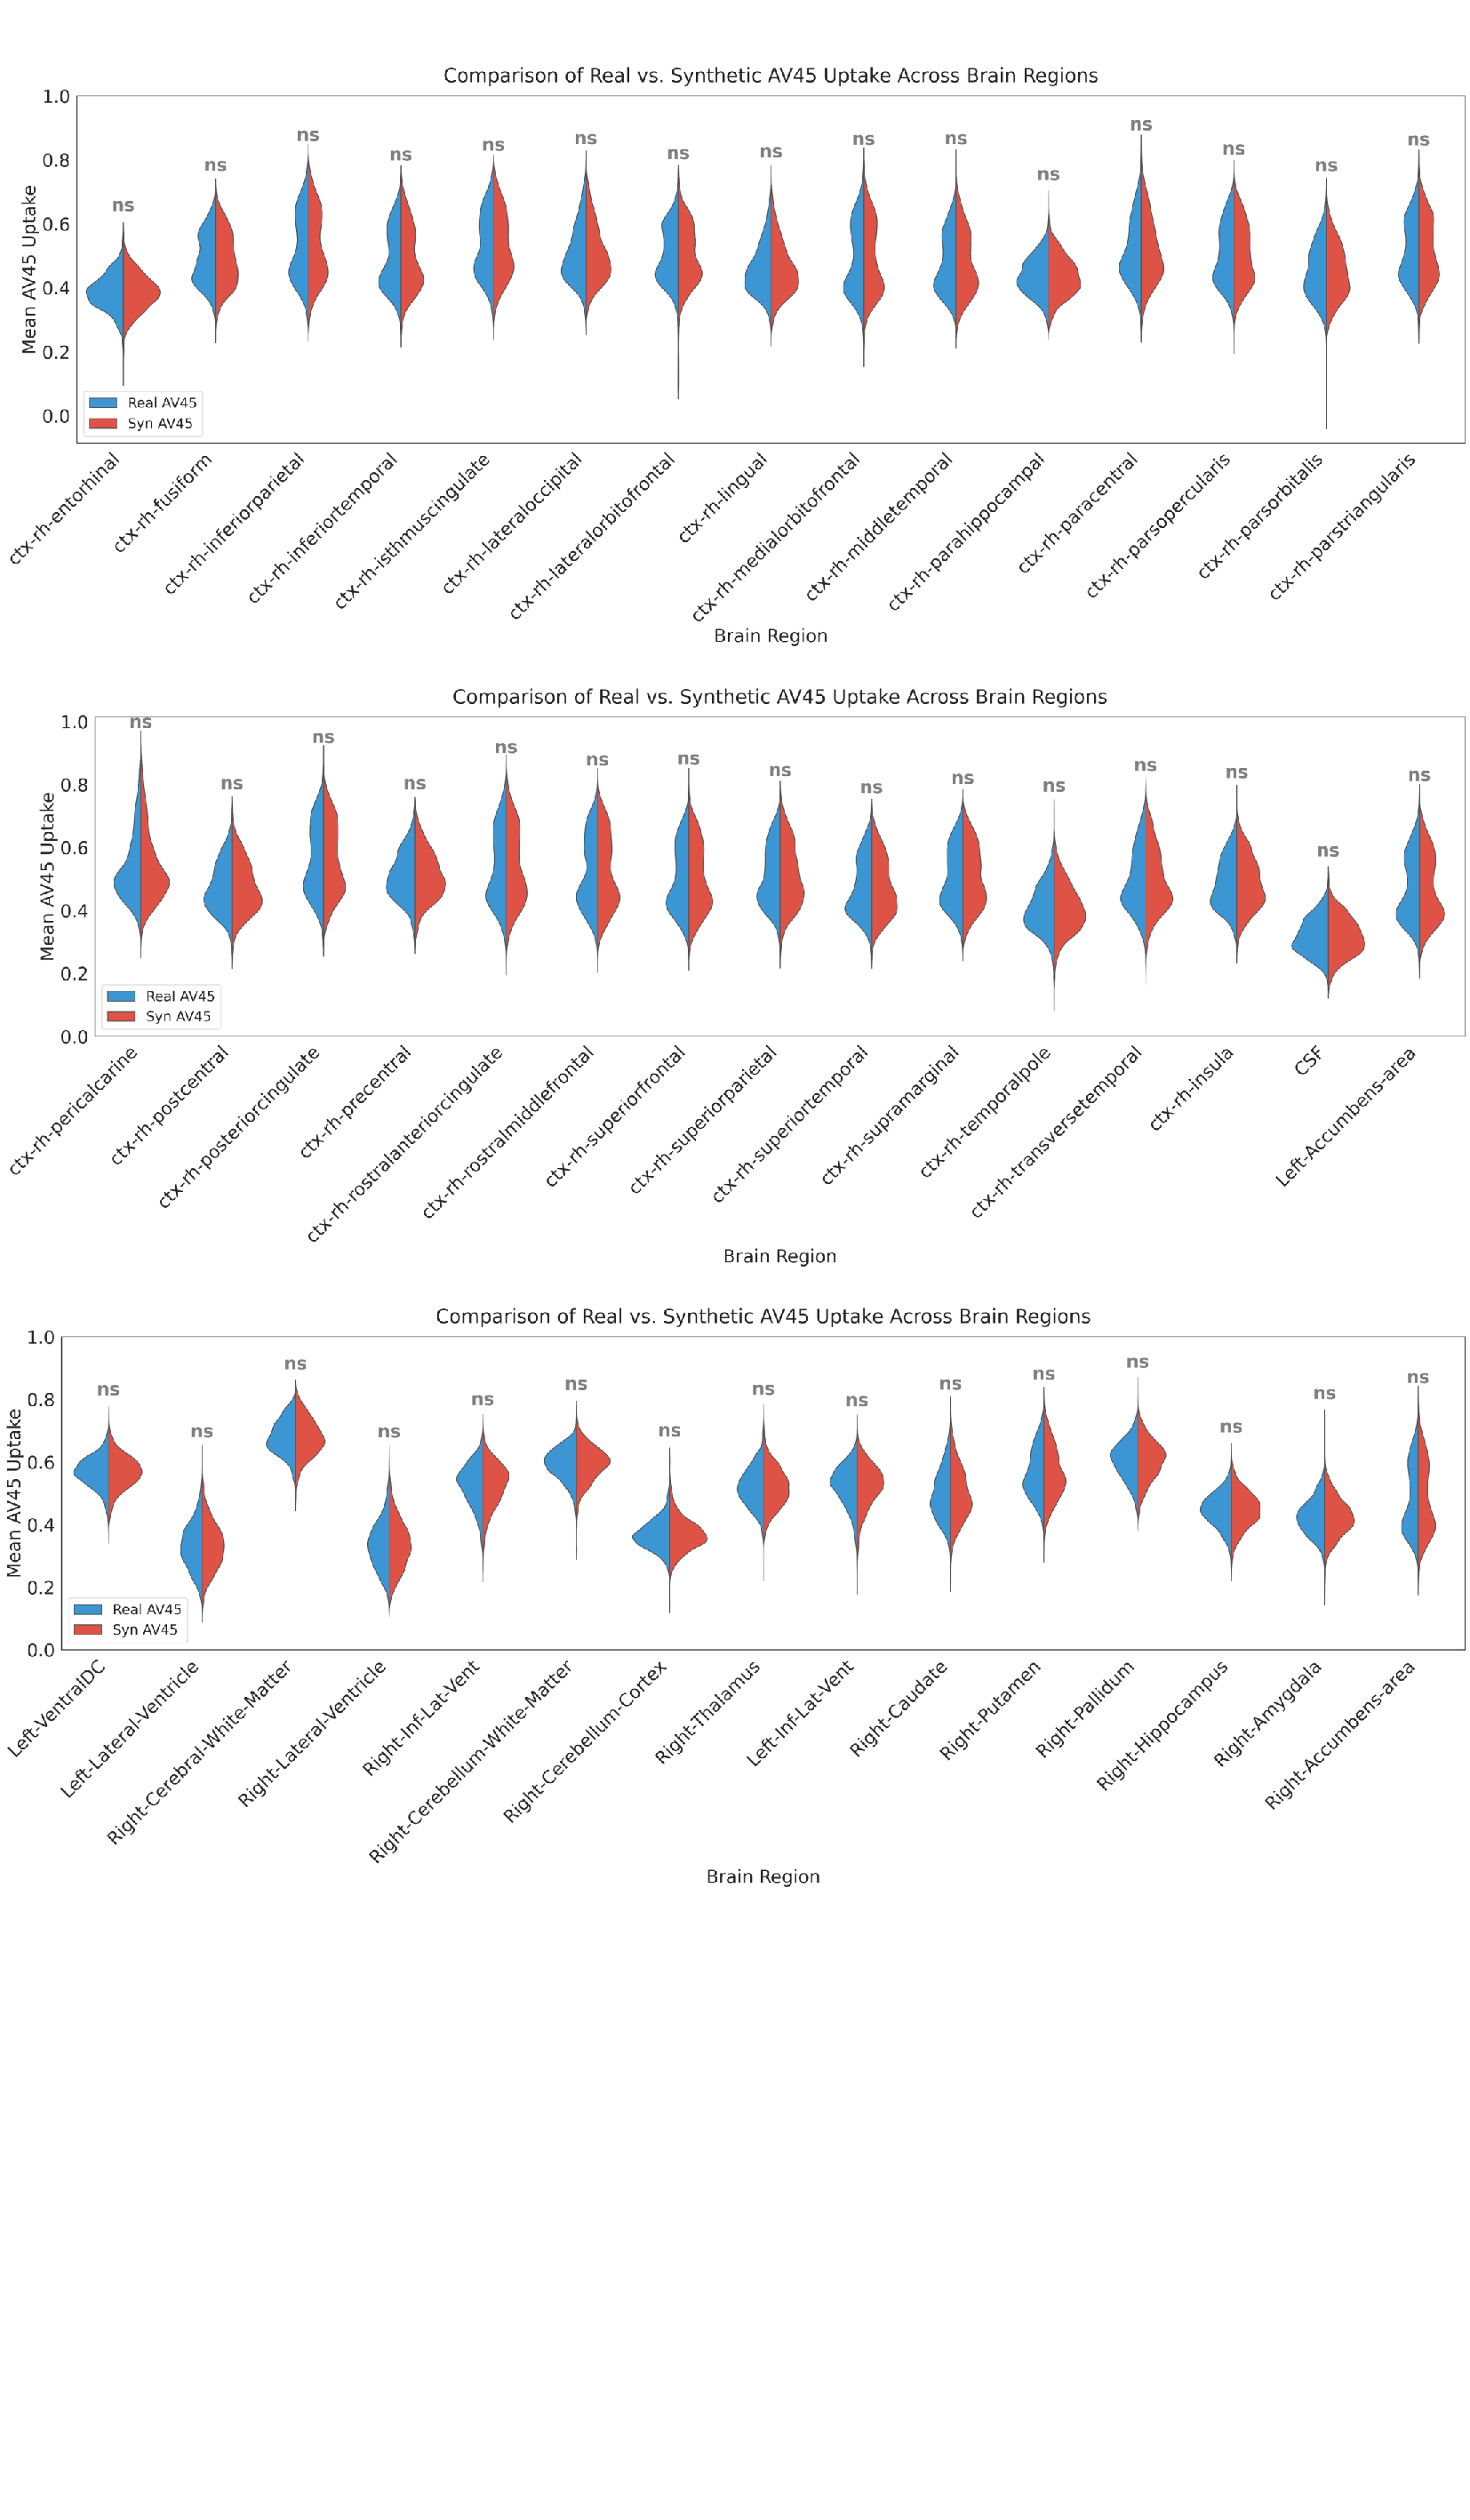
\includegraphics[width=\textwidth]{supplementary_figure_2}
    \caption{\textbf{Comparison of real and synthetic AV45 uptake across the remaining brain regions (Part 2 of 2).}}
    \label{fig:supp_av45_2}
\end{figure}

\begin{figure}[htbp]
    \centering
    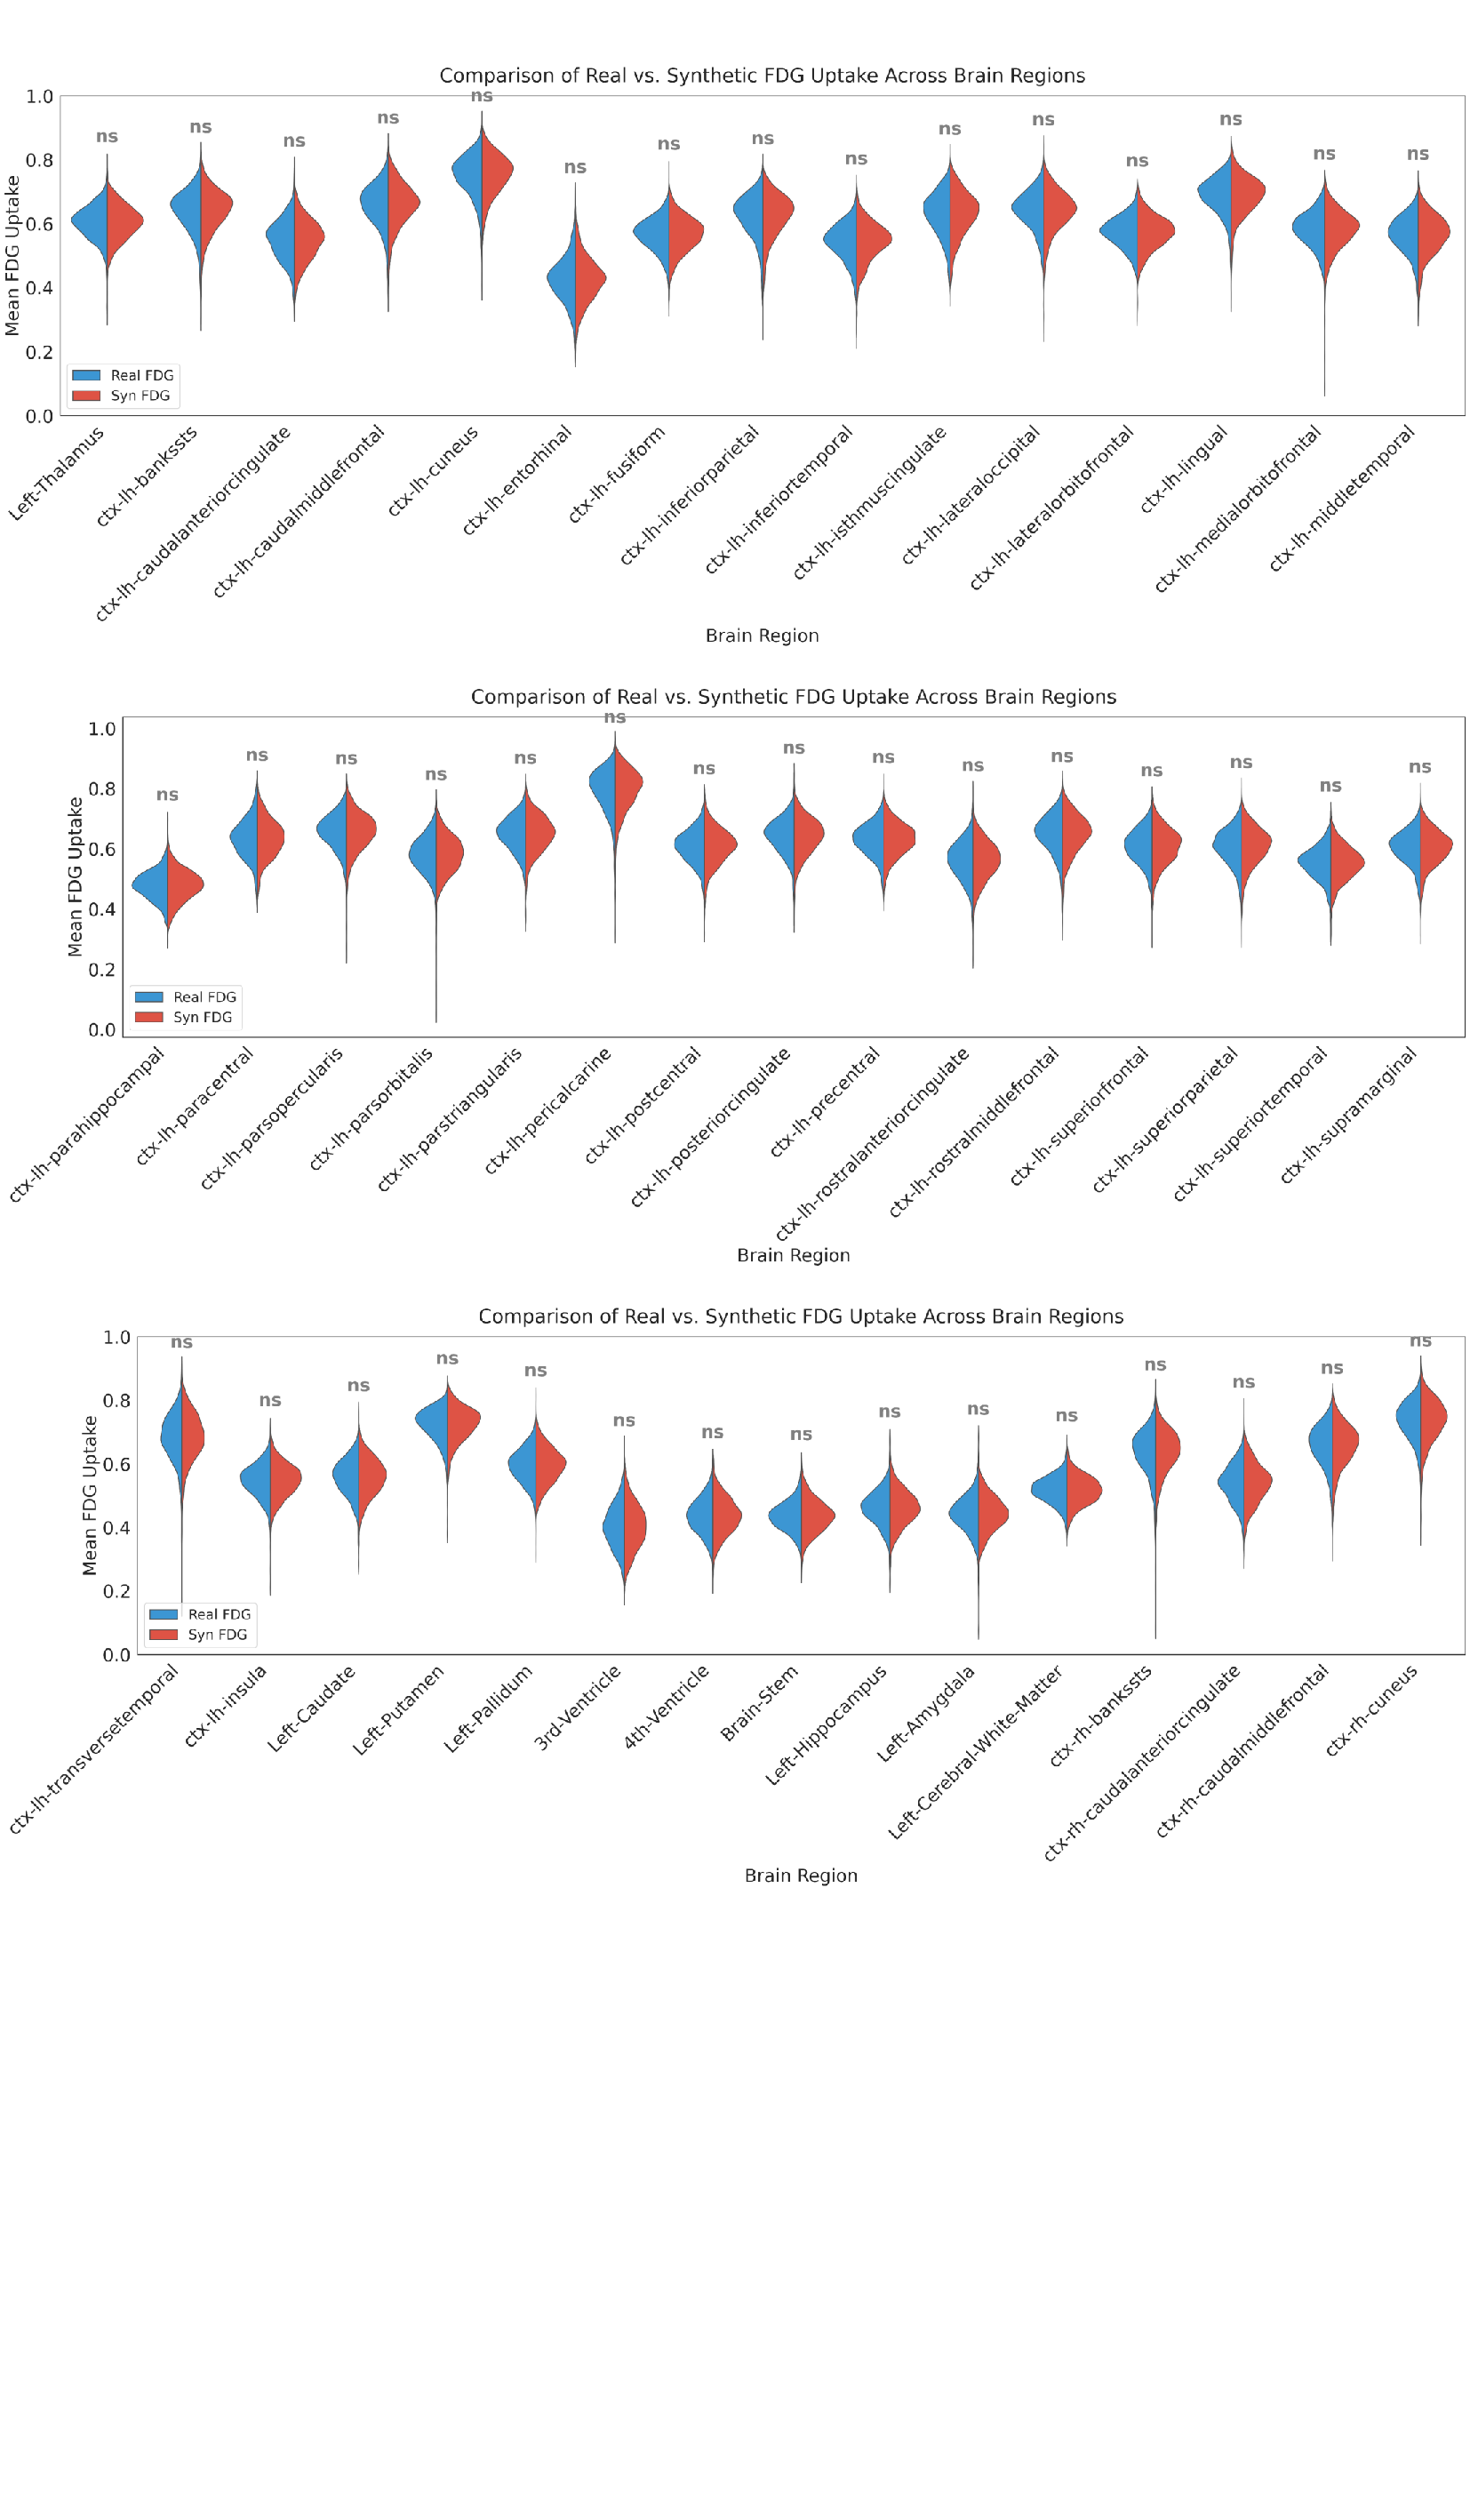
\includegraphics[width=\textwidth]{supplementary_figure_3}
    \caption{\textbf{Comparison of real and synthetic FDG uptake across the remaining brain regions (Part 1 of 2).}}
    \label{fig:supp_fdg_1}
\end{figure}

\begin{figure}[htbp]
    \centering
    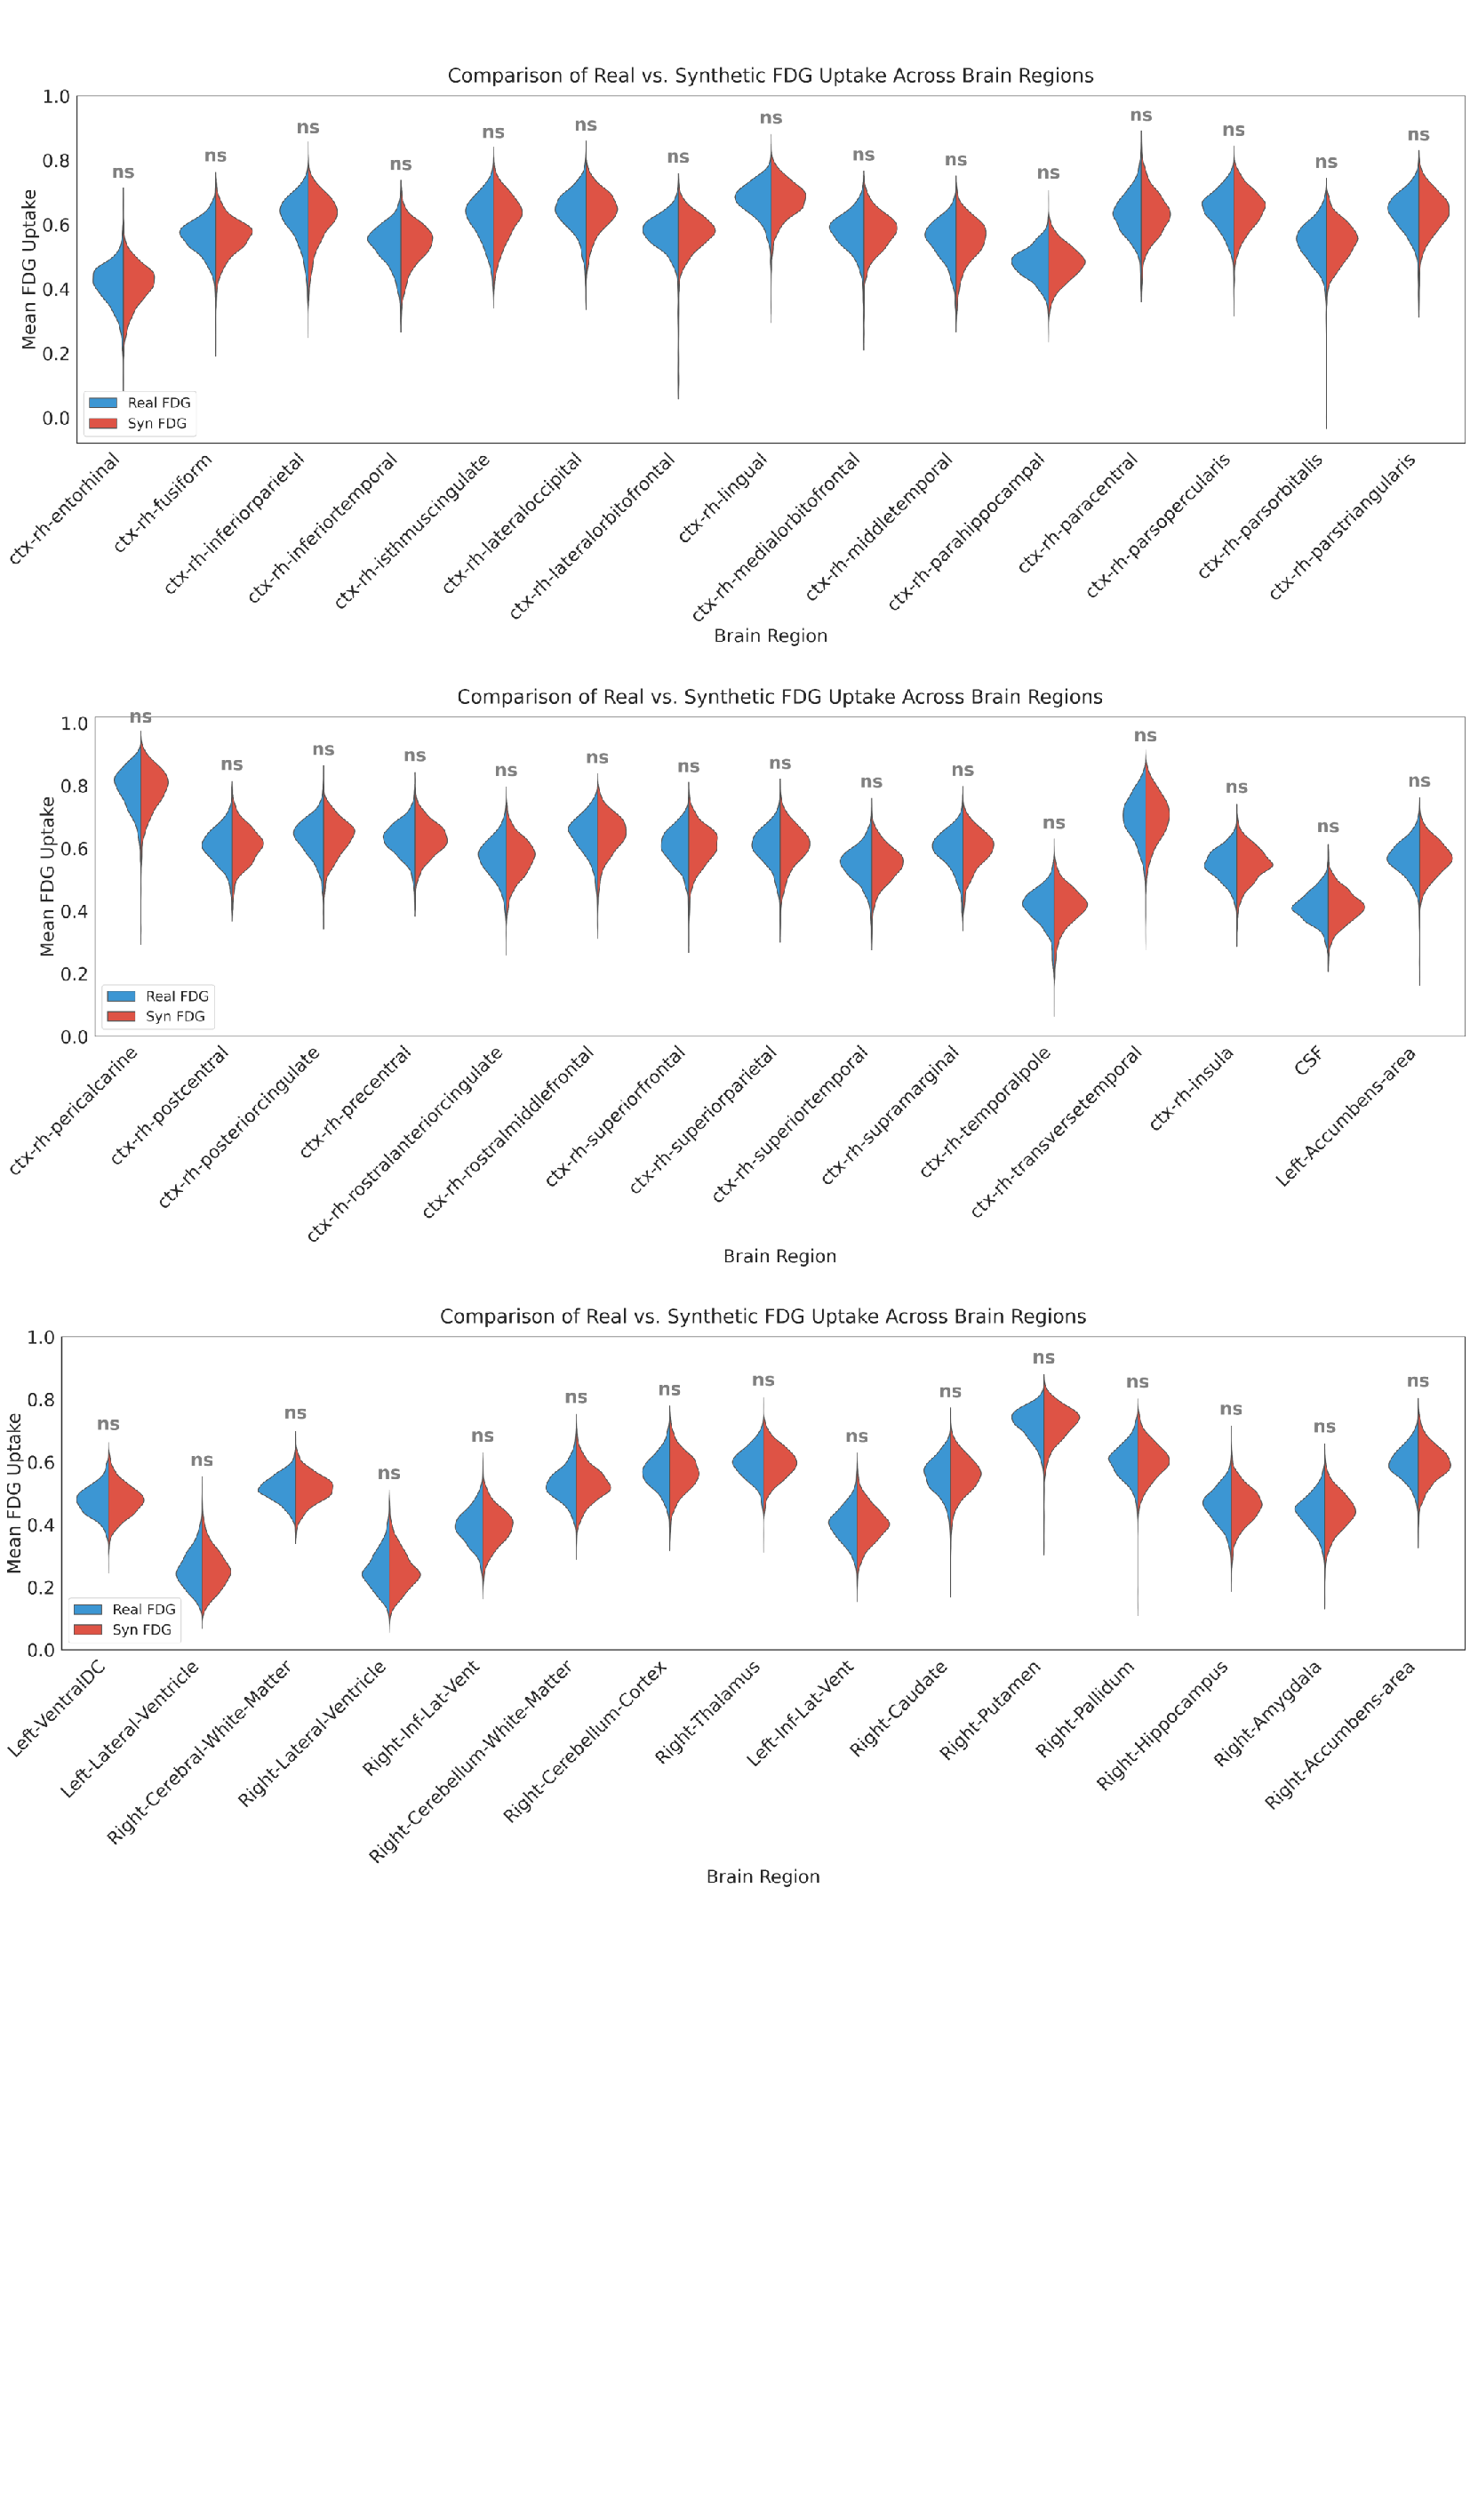
\includegraphics[width=\textwidth]{supplementary_figure_4}
    \caption{\textbf{Comparison of real and synthetic FDG uptake across the remaining brain regions (Part 2 of 2).}}
    \label{fig:supp_fdg_2}
\end{figure}

\begin{figure}[htbp]
    \centering
    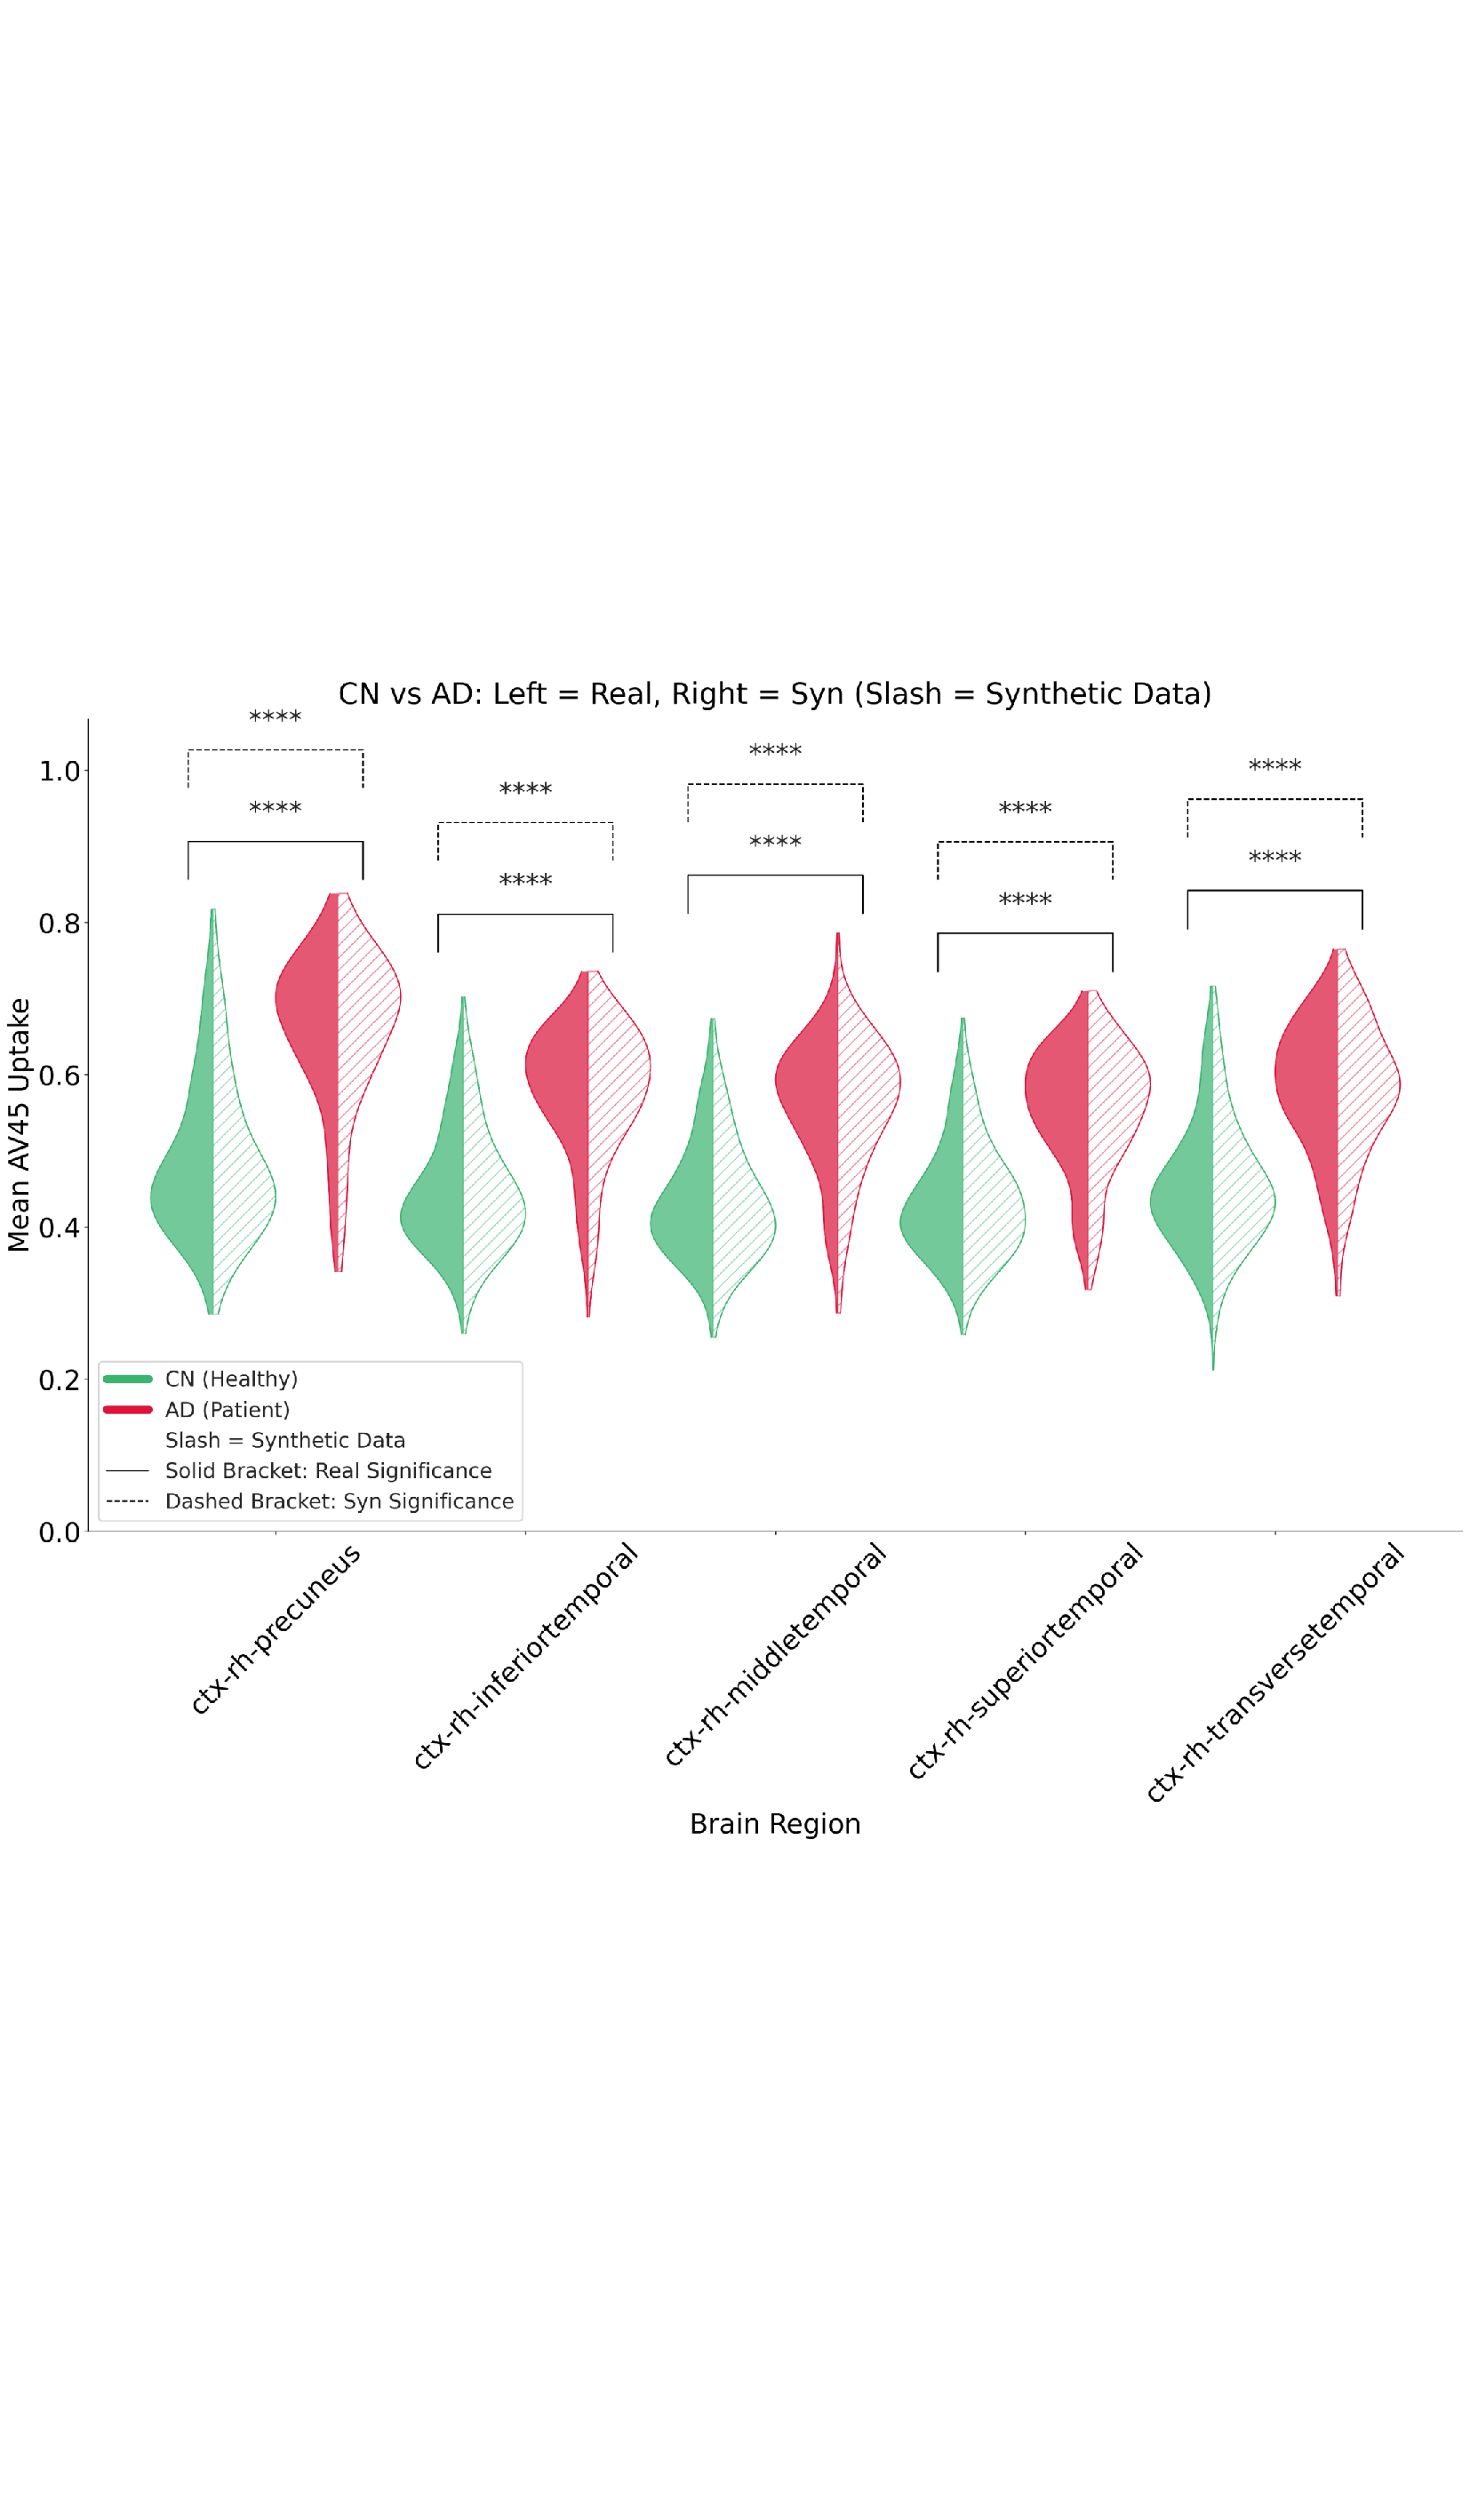
\includegraphics[width=\textwidth]{supplementary_figure_5}
    \caption{\textbf{Validation of disease-related AV45 uptake patterns across the remaining brain regions.} Violin plots display mean uptake in Alzheimer’s disease (AD, red) and cognitively normal (CN, green) subjects for selected brain regions. Each region contains paired half-violins: the left half (solid fill) represents real PET data, and the right half (dashed fill) represents MRI-synthetic PET data, with consistent color coding between modalities. Solid lines above the violins indicate statistical significance for real PET, while dashed lines indicate significance for synthetic PET.}
    \label{fig:supp_disease_av45}
\end{figure}

\begin{figure}[htbp]
    \centering
    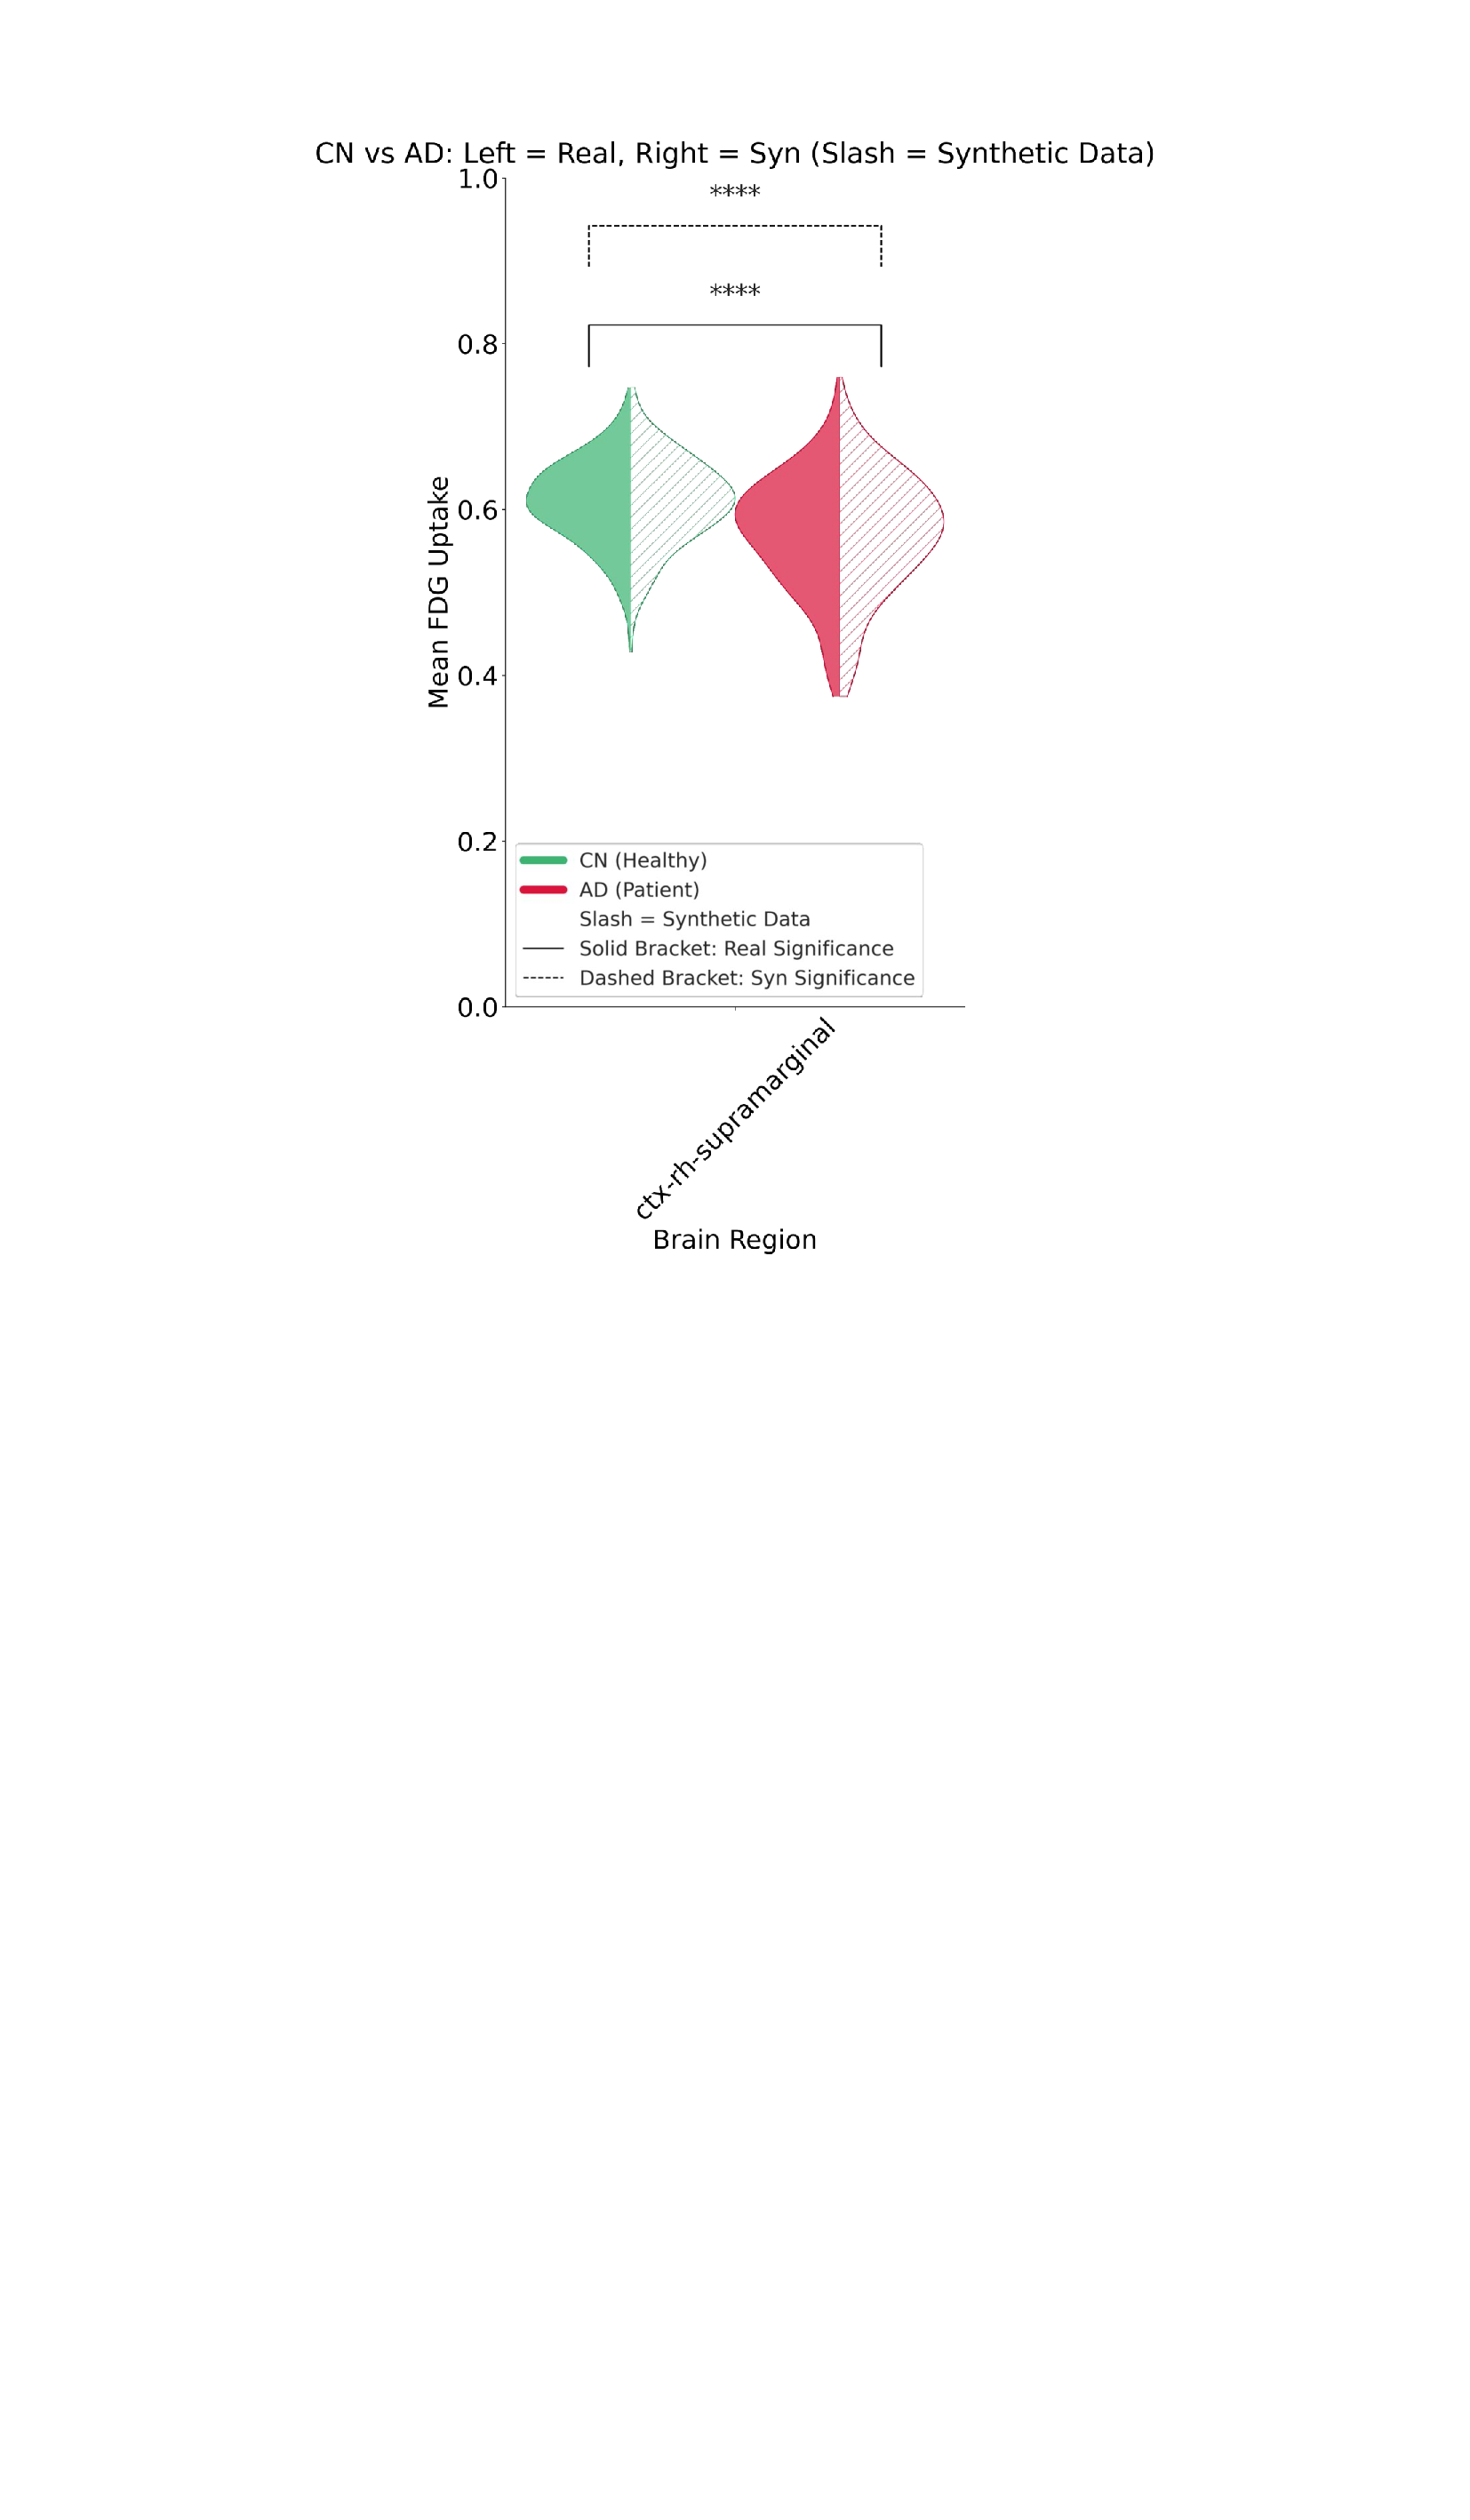
\includegraphics[width=0.75\textwidth]{supplementary_figure_6}
    \caption{\textbf{Validation of disease-related FDG uptake patterns across the remaining brain regions.} Violin plots display mean uptake in Alzheimer’s disease (AD, red) and cognitively normal (CN, green) subjects for selected brain regions. Each region contains paired half-violins: the left half (solid fill) represents real PET data, and the right half (dashed fill) represents MRI-synthetic PET data, with consistent color coding between modalities. Solid lines above the violins indicate statistical significance for real PET, while dashed lines indicate significance for synthetic PET.}
    \label{fig:supp_disease_fdg}
\end{figure}

\begin{table}[htbp]
\caption{\textbf{Demographic characteristics of ADNI.} Data are mean $\pm$ s.d. unless otherwise indicated. $P$ values from one-way ANOVA (continuous) or chi-square test (sex). CDR: Clinical Dementia Rating; MMSE: Mini-Mental State Examination.}
\label{tab:supp_adni}
\centering
\begin{tabularx}{\textwidth}{l *{5}{>{\centering\arraybackslash}X} >{\centering\arraybackslash}X}
\toprule
 & \textbf{CN} & \textbf{EMCI} & \textbf{LMCI} & \textbf{MCI} & \textbf{AD} & \textbf{P} \\
\midrule
$n$ & 577 & 291 & 152 & 520 & 317 & \\
Age (years) & 72.55 $\pm$ 6.65 & 71.62 $\pm$ 7.51 & 72.44 $\pm$ 7.69 & 73.20 $\pm$ 7.51 & 74.90 $\pm$ 7.99 & $<$0.001 \\
Weight (kg) & 73.20 $\pm$ 24.13 & 80.77 $\pm$ 16.67 & 77.15 $\pm$ 16.64 & 72.90 $\pm$ 22.33 & 73.21 $\pm$ 18.64 & 0.0023 \\
Sex (M/F) & 252/325 & 165/126 & 80/72 & 310/210 & 186/131 & $<$0.001 \\
MMSE & 29.40 $\pm$ 0.70 & 27.50 $\pm$ 0.50 & 24.47 $\pm$ 0.50 & 26.83 $\pm$ 1.24 & 20.84 $\pm$ 1.97 & $<$0.001 \\
GDSCALE & 0.24 $\pm$ 0.73 & 1.01 $\pm$ 0.14 & 3.02 $\pm$ 0.28 & 1.81 $\pm$ 0.99 & 4.14 $\pm$ 1.62 & $<$0.001 \\
Global CDR & 0.00 $\pm$ 0.02 & 0.15 $\pm$ 0.23 & 0.50 $\pm$ 0.01 & 0.42 $\pm$ 0.19 & 0.95 $\pm$ 0.15 & $<$0.001 \\
FAQ & 0.52 $\pm$ 0.53 & 3.11 $\pm$ 2.42 & 8.83 $\pm$ 1.54 & 5.33 $\pm$ 1.51 & 20.20 $\pm$ 2.92 & $<$0.001 \\
NPI-Q & 0.01 $\pm$ 0.19 & 1.55 $\pm$ 2.17 & 4.00 $\pm$ 0.03 & 2.92 $\pm$ 0.50 & 4.98 $\pm$ 0.65 & $<$0.001 \\
\bottomrule
\end{tabularx}

\vspace{2mm}
\footnotesize
\textit{Note:} CN = Cognitively Normal; EMCI = Early MCI; LMCI = Late MCI; MCI = Mild Cognitive Impairment; AD = Alzheimer’s dementia.
\end{table}

To obtain the required text-guided information for our analysis, we performed secondary screening within the OASIS-3 cohort (Open Access Series of Imaging Studies), a longitudinal neuroimaging, clinical, and cognitive dataset for normal aging and Alzheimer’s disease (available at: \url{https://www.medrxiv.org/content/10.1101/2019.12.13.19014902v1.full.pdf}). We focused on individuals with amyloid-beta PET imaging data processed through the standardized Pet Unified Pipeline (PUP). Specifically, we selected 419 participants who had undergone AV45 PET scans and were PUP-processed, ensuring high-quality, quantitatively reliable neuroimaging data. These individuals formed the basis of our subsequent multimodal analysis. In contrast, FDG-PET data from a smaller subset ($n = 117$) were not processed with the PUP pipeline and were therefore excluded to maintain methodological consistency. The demographic characteristics of this selected cohort, including age and gender distribution, are detailed in Table~\ref{tab:supp_oasis}.

\begin{table}[htbp]
\caption{\textbf{Demographic characteristics of OASIS-3.}}
\label{tab:supp_oasis}
\centering
\begin{tabularx}{\textwidth}{l *{3}{>{\centering\arraybackslash}X}}
\toprule
 & \textbf{CN} & \textbf{AD} & \textbf{P} \\
\midrule
$n$ & 334 & 85 & \\
Age (years) & 66.33 $\pm$ 8.38 & 72.76 $\pm$ 6.96 & $<$0.001 \\
Sex (M/F) & 143/191 & 37/48 & $>$0.05 \\
MMSE score & 29.24 $\pm$ 0.90 & 23.21 $\pm$ 3.51 & $<$0.001 \\
Global CDR & 0.01 $\pm$ 0.08 & 0.73 $\pm$ 0.59 & $<$0.001 \\
\bottomrule
\end{tabularx}

\vspace{2mm}
\footnotesize
\textit{Note:} CN = Cognitively Normal; AD = Alzheimer’s dementia.
\end{table}

\begin{table}[htbp]
\caption{\textbf{Core software dependencies and versions for DIReCT$++$.} Only packages directly relevant to model implementation, training, and evaluation are listed. Full environment details are available in the code repository.}
\label{tab:supp_software}
\centering
\begin{tabularx}{\textwidth}{lX lX}
\toprule
\textbf{Package} & \textbf{Version} & \textbf{Package} & \textbf{Version} \\
\midrule
Python & 3.10 & PyTorch & 2.6.0+cu118 \\
torchvision & 0.21.0+cu118 & torchaudio & 2.6.0+cu118 \\
CUDA & 11.8 & cuDNN & 9.1.0 \\
einops & 0.8.1 & transformers & 4.40.2 \\
tokenizers & 0.19.1 & safetensors & 0.5.3 \\
xformers & 0.0.29.post3 & faiss & 1.9.0 \\
monai & 1.5.1 & numpy & 2.2.4 \\
scipy & 1.15.2 & pandas & 2.2.3 \\
scikit-learn & 1.6.1 & matplotlib & 3.10.1 \\
seaborn & 0.13.2 & opencv-python & 4.12.0.88 \\
nibabel & 5.3.2 & tensorboard & 2.19.0 \\
fsspec & 2024.6.1 & huggingface-hub & 0.30.1 \\
protobuf & 6.30.2 & triton & 3.2.0 \\
\bottomrule
\end{tabularx}
\end{table}
